\documentclass[a4paper,12pt]{article} % добавить leqno в [] для нумерации слева
\usepackage[a4paper,top=1.3cm,bottom=2cm,left=1.5cm,right=1.5cm,marginparwidth=0.75cm]{geometry}
%%% Работа с русским языком
\usepackage{cmap}					% поиск в PDF
\usepackage[warn]{mathtext} 		% русские буквы в фомулах
\usepackage[T2A]{fontenc}			% кодировка
\usepackage[utf8]{inputenc}			% кодировка исходного текста
\usepackage[english,russian]{babel}	% локализация и переносы
\usepackage{physics}
\usepackage{multirow}
\usepackage{longtable}

%%% Нормальное размещение таблиц (писать [H] в окружении таблицы)
\usepackage{float}
\restylefloat{table}



\usepackage{graphicx}

\usepackage{wrapfig}
\usepackage{tabularx}

\usepackage{hyperref}
\usepackage[rgb]{xcolor}
\hypersetup{
	colorlinks=true,urlcolor=blue
}

\usepackage{pgfplots}
\pgfplotsset{compat=1.9}

%%% Дополнительная работа с математикой
\usepackage{amsmath,amsfonts,amssymb,amsthm,mathtools} % AMS
\usepackage{icomma} % "Умная" запятая: $0,2$ --- число, $0, 2$ --- перечисление

%% Номера формул
\mathtoolsset{showonlyrefs=true} % Показывать номера только у тех формул, на которые есть \eqref{} в тексте.

%% Шрифты
\usepackage{euscript}	 % Шрифт Евклид
\usepackage{mathrsfs} % Красивый матшрифт

%% Свои команды
\DeclareMathOperator{\sgn}{\mathop{sgn}}

%% Перенос знаков в формулах (по Львовскому)
\newcommand*{\hm}[1]{#1\nobreak\discretionary{}
	{\hbox{$\mathsurround=0pt #1$}}{}}

\date{\today}

\usepackage{gensymb}

\begin{document}

\begin{titlepage}
	\begin{center}
		{\large МОСКОВСКИЙ ФИЗИКО-ТЕХНИЧЕСКИЙ ИНСТИТУТ (НАЦИОНАЛЬНЫЙ ИССЛЕДОВАТЕЛЬСКИЙ УНИВЕРСИТЕТ)}
	\end{center}
	\begin{center}
		{\large Физтех-школа физики и исследований им. Ландау}
	\end{center}
	
	
	\vspace{4.5cm}
	{\huge
		\begin{center}
			{\bf Отчёт о выполнении лабораторной работы 2.1.3}\\
			Определение $ C_p/C_v $ по скорости звука в газе
		\end{center}
	}
	\vspace{2cm}
	\begin{flushright}
		{\LARGE Автор:\\ Сенокосов Арсений Олегович \\
			\vspace{0.2cm}
			Б02-012}
	\end{flushright}
	\vspace{8cm}
	\begin{center}
		Долгопрудный\\
		\today
	\end{center}
\end{titlepage}


\section{Введение}
\textbf{Цель работы:}  \begin{enumerate}
\item измерение частоты колебаний и длины волны при резонансе звуковых колебаний в газе, заполняющем трубу;
\item определение показателя адиабаты с помощью уравнения состояния идеального газа.
\end{enumerate}

\textbf{В работе используются:} звуковой генератор ГЗ; электронный осциллограф ЭО; микрофон; телефон; раздвижная труба; теплоизолированная труба, обогреваемая водой из термостата; баллон со сжатым углекислым газом; газгольдер.

\section{Теоретические сведения}

Скорость распространения звуковой волны в газах зависит от показателя адиабаты $ \gamma $. На измерении скорости звука основан один из наиболее точных методов определения показателя адиабаты.

Скорость звука в газах определяется формулой:

\begin{equation}\label{velocity}
c=\sqrt{\gamma\frac{RT}{\mu}}.
\end{equation}
где $ R $ -- газовая постоянная, $ T $ -- температура газа, а $ \mu $ -- его молярная масса. Преобразуя эту формулу, найдем
\begin{equation}\label{gamma}
\boxed{\gamma = \frac{\mu}{RT}c^2}.
\end{equation}

Таким образом, для определения показателя адиабаты достаточно измерить температуру газа и скорость распространения звука (молярная масса газа предполагается известной).

Звуковая волна, распространяющаяся вдоль трубы, испытывает многократные отражения от торцов. Звуковые колебания в трубе являются наложением всех отраженных волн и очень сложны. Картина упрощается, если длина трубы $ L $ равна целому числу полуволн, то есть когда \[ L=n\lambda/2, \] где $ \lambda $ -- длина волны звука в трубе, а $ n $ -- любое целое число. Если это условие выполнено, то волна, отраженная от торца трубы, вернувшаяся к ее началу и вновь отраженная, совпадает по фазе с падающей. Совпадающие по фазе волны усиливают друг друга. Амплитуда звуковых колебаний при этом резко возрастает -- наступает резонанс.

При звуковых колебаниях слои газа, прилегающие к торцам трубы, не испытывают смещения. Узлы смещения повторяются по всей длине трубы через $ \lambda/2 $. Между узлами находятся максимумы смещения.

Скорость звука c связана с его частотой $ f $ и длиной волны $ \lambda $ соотношением

\begin{equation}\label{lambda_f}
c=\lambda f.
\end{equation}

Подбор условий, при которых возникает резонанс, можно производить двояко:
\begin{enumerate}
	\item При неизменной частоте $ f $ звукового генератора (а следовательно, и неизменной длине звуковой волны $ \lambda $) можно изменять длину трубы $ L $. Для этого применяется раздвижная труба. Длина раздвижной трубы постепенно увеличивается, и наблюдается ряд последовательных резонансов. Возникновение резонанса легко наблюдать на осциллографе по резкому увеличению амплитуды колебаний. Для последовательных резонансов имеем \begin{equation}\label{first}
	L_n=n\frac{\lambda}{2}, \quad L_{n+1}=(n+1)\frac{\lambda}{2}, \quad \dots, \quad L_{n+k} = n\frac{\lambda}{2}+k\frac{\lambda}{2},
	\end{equation} т. е. $ \lambda/2 $ равно угловому коэффициенту графика, изображающего зависимость длины трубы $ L $ от номера резонанса $ k $. Скорость звука находится по формуле \eqref{lambda_f}.
	\item При постоянной длине трубы можно изменять частоту звуковых колебаний. В этом случае следует плавно изменять частоту $ f $ звукового генератора, а следовательно, и длину звуковой волны $ \lambda $. Для последовательных резонансов получим 
	\begin{equation}\label{4}
	L=\frac{\lambda_1}{2}n=\frac{\lambda_2}{2}(n+1)=\dots=\frac{\lambda_{k+1}}{2}(n+k).
	\end{equation}
	
	Из \eqref{lambda_f} и \eqref{4} имеем:
	\[ f_1=\frac{c}{\lambda_1}=\frac{c}{2L}n, \quad f_2=\frac{c}{\lambda_2}=\frac{c}{2L}(n+1)=f_1+\frac{c}{2L},\quad \dots, \]
	\begin{equation}\label{5}
	f_{k+1}=\frac{c}{\lambda_{k+1}}=\frac{c}{2L}(n+k)=f_1+\frac{c}{2L}k.
	\end{equation}
	Скорость звука, деленная на $ 2L $, определяется, таким образом, по угловому коэффициенту графика зависимости частоты от номера резонанса.
\end{enumerate}

\section{Экспериментальная установка}

Соответственно двум методам измерения скорости звука в работе имеются две установки (рис. \ref{img1} и \ref{img2}). В обеих установках звуковые колебания в трубе возбуждаются телефоном Т и улавливаются микрофоном М. Мембрана телефона приводится в движение переменным током звуковой частоты; в качестве источника переменной ЭДС используется звуковой генератор ГЗ. Возникающий в микрофоне сигнал наблюдается на осциллографе ЭО.

Микрофон и телефон присоединены к установке через тонкие резиновые трубки. Такая связь достаточна для возбуждения и обнаружения звуковых колебаний в трубе и в то же время мало возмущает эти колебания: при расчетах оба торца трубы можно считать неподвижными, а влиянием соединительных отверстий пренебречь.

Первая установка (рис. \ref{img1}) содержит раздвижную трубу с миллиметровой шкалой. Через патрубок (на рисунке не показан) труба может наполняться воздухом или углекислым газом из газгольдера. На этой установке производятся измерения $ \gamma $ для воздуха и для $ CO_2 $. Вторая установка (рис. \ref{img2}) содержит теплоизолированную трубу постоянной длины. Воздух в трубе нагревается водой из термостата. Температура газа принимается равной температуре омывающей трубу воды. На этой установке измеряется зависимость скорости звука от температуры.

\begin{figure}[H]
	\begin{center}
		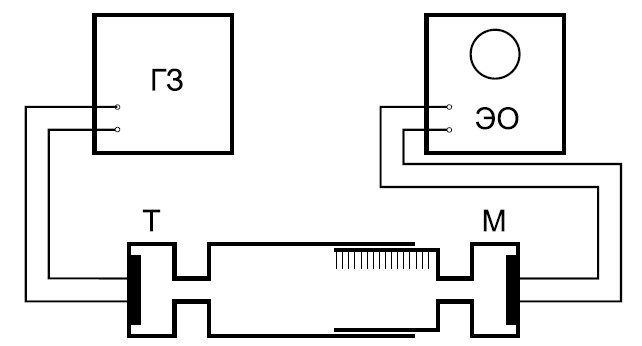
\includegraphics[width=12cm]{ust1.jpg}
	\end{center}
	\caption{\textit{Установка для измерения скорости звука при помощи раздвижной трубы}}
	\label{img1}
\end{figure}

\begin{figure}[H]
	\begin{center}
		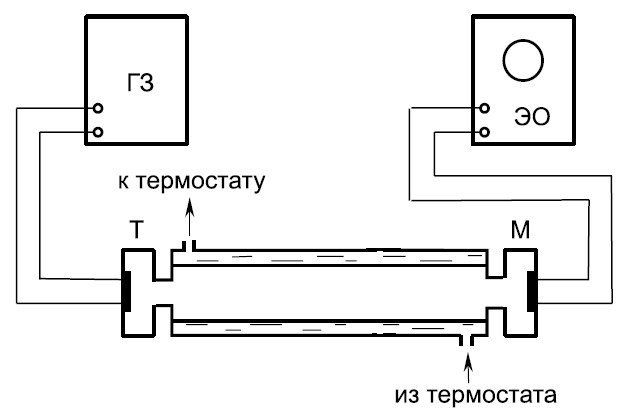
\includegraphics[width=12cm]{ust2.jpg}
	\end{center}
	\caption{\textit{Установка для изучения зависимости скорости звука от температуры}}
	\label{img2}
\end{figure}

\section{Ход работы}

\subsection{Измерение $ C_p/C_v $ для воздуха при помощи установки с раздвижной трубой}

\label{ident}

Проведём измерение коэффициента $ C_p/C_v $ для воздуха при помощи установки с раздвижной трубой. Для проведения серии измерений фиксируем частоту звукового сигнала и оставляем её неизменной при до окончания снятия показаний. Увеличиваем и уменьшаем длину трубки, чтобы добиться резонанса, возникновение которого устанавливается при помощи осциллографа. При возникновении резонанса фиксируем то расстояние, на которое была выдвинута трубка прибора. Данные измерения проводим для нескольких значений частот. Полученные результаты заносим в таблицу \ref{tab:oxy}.

\begin{table}[H]
	\centering
	\begin{tabular}{|c|c|c|c|c|c|c|c|c|c|c|}
		\hline
		$ f $, Гц & \multicolumn{2}{c|}{\textbf{2700}} & \multicolumn{2}{c|}{\textbf{2998}} & \multicolumn{2}{c|}{\textbf{3502}} & \multicolumn{2}{c|}{\textbf{4042}} & \multicolumn{2}{c|}{\textbf{4476}} \\ \hline
		$ k $ & $ l_k $, мм & $ L_k $, мм & $ l_k $, мм & $ L_k $, мм & $ l_k $, мм & $ L_k $, мм & $ l_k $, мм & $ L_k $, мм & $ l_k $, мм & $ L_k $, мм \\ \hline
		0 & 13 & 0 & 7 & 0 & 25 & 0 & 34 & 0 & 14 & 0 \\ \hline
		1 & 76 & 63 & 65 & 58 & 75 & 50 & 77 & 43 & 52 & 38 \\ \hline
		2 & 140 & 127 & 122 & 115 & 124 & 99 & 120 & 86 & 90 & 76 \\ \hline
		3 & 205 & 192 & 180 & 173 & 174 & 149 & 162 & 128 & 129 & 115 \\ \hline
		4 &  &  &  &  & 224 & 199 & 205 & 171 & 167 & 153 \\ \hline
		5 &  &  &  &  &  &  &  &  & 206 & 192 \\ \hline
	\end{tabular}
	\caption{Результаты измерений для воздуха}
	\label{tab:oxy}
\end{table}

Для каждого измерения величины <<выдвига>> трубы $ \sigma_l = 0,5 $ мм. Также для каждого измерения вычислим $ L_k = l_k - l_0 $. Погрешность определения этой величины составит $ \sigma_L=~\sqrt{2}\sigma_l \approx~0,7 $~мм.

По полученным данным построим графики зависимости $ L_k(k) $.

Аппроксимируем полученные зависимости прямыми $ y=ax $ используя метод наименьших квадратов. Коэффициент $ a $ находим согласно следующей формуле:

\begin{equation}\label{mnk:a}
a=\frac{\left\langle kL_k \right\rangle}{\left\langle k^2 \right\rangle}.
\end{equation}

\begin{center}
	\begin{tikzpicture}
	\begin{axis}[
	title={График зависимости $L_k(k)$ для воздуха},
	xlabel={Номера резонанса $ k $},
	ylabel={Величина <<выдвига>> $ L_k $, мм},
	legend pos=north west,
	xmajorgrids=true,
	ymajorgrids=true,
	grid style=dashed,
	/pgf/number format/.cd,%
	set thousands separator={},
	set decimal separator={,},
	xmin = 0,
	xmax = 5.3,
	ymin = 0,
	%ymax = 5500,
	width = 530,
	height = 320,
	]
	\legend{ 
		$ f = 2700 $ Гц,,
		$ f = 2998 $ Гц,,
		$ f = 3502 $ Гц,,
		$ f = 4042 $ Гц,,
		$ f = 4476 $ Гц,,
	};

	\addplot+ [black, only marks, mark size = 3pt,
	mark=*, 
	mark options = {
		fill = red, 
		draw = black},
	error bars/.cd,
	y dir=both, y explicit,
	] table [x = k, y = L, y error = dL,] {
		k	L	dL
		0	0	0.707106781
		1	63	0.707106781
		2	127	0.707106781
		3	192	0.707106781
	};
	\addplot [red, domain=0:3.1, line width = 2.2pt] { 63.78571421 * x};
	
	\addplot+ [black, only marks, mark size = 3pt, 
	mark options = {
		fill = blue, 
		draw = black},
	error bars/.cd,
	y dir=both, y explicit,
	] table [x = k, y = L, y error = dL,] {
		k	L	dL
		0	0	0.707106781
		1	58	0.707106781
		2	115	0.707106781
		3	173	0.707106781
	};
	\addplot [blue, domain=0:3.1, line width = 2.2pt] { 57.6428571343983 * x};
	
	\addplot+ [black, only marks, mark size = 3pt, 
	mark options = {
		fill = green, 
		draw = black},
	error bars/.cd,
	y dir=both, y explicit,
	] table [x = k, y = L, y error = dL,] {
		k	L	dL
		0	0	0.707106781
		1	50	0.707106781
		2	99	0.707106781
		3	149	0.707106781
		4	199	0.707106781
	};
	\addplot [green, domain=0:4.1, line width = 2.2pt] { 49.7000000055265 * x};
	
	\addplot+ [black, only marks, mark size = 3pt, 
	mark options = {
		fill = orange, 
		draw = black},
	error bars/.cd,
	y dir=both, y explicit,
	] table [x = k, y = L, y error = dL,] {
		k	L	dL
		0	0	0.707106781
		1	43	0.707106781
		2	86	0.707106781
		3	128	0.707106781
		4	171	0.707106781
		
	};
	\addplot [orange, domain=0:4.1, line width = 2.2pt] { 42.7666666832461 * x};
	
	\addplot+ [black, mark=halfcircle*, only marks, mark size = 3pt, 
	mark options = {
		fill = violet, 
		draw = black},
	error bars/.cd,
	y dir=both, y explicit,
	] table [x = k, y = L, y error = dL,] {
		k	L	dL
		0	0	0.707106781
		1	38	0.707106781
		2	76	0.707106781
		3	115	0.707106781
		4	153	0.707106781
		5	192	0.707106781
		
	};
	\addplot [violet, domain=0:5.1, line width = 2.2pt] { 38.3090909333986 * x};
	
	\end{axis}
	\end{tikzpicture}
\end{center}

Случайную погрешность определения $ a $ оценим следующим образом:

\begin{equation}\label{mnk:sigma_a}
\sigma^\text{случ}_a=\sqrt{\frac{1}{N-1}\left(\frac{\left\langle L_k^2 \right\rangle}{\left\langle k^2 \right\rangle}-a^2\right)},
\end{equation}
где $ N $ -- колличество измерений. Систематическая погрешность определения $ a $ равна $ \sigma_a^\text{сист} = \sigma_{L_k} $. Тогда полная погрешность определения коэффициента $ a $ может быть вычислена по следующей формуле:

\begin{equation}\label{mnk:full_sigma}
\sigma_a=\sqrt{\left(\sigma^\text{случ}_a\right)^2+\left(\sigma^\text{сист}_a\right)^2}.
\end{equation}

Используя эти формулы вычисляем коэффициенты $ a $ для каждого значения частоты $ f $. результаты вычислений заносим в таблицу \ref{tab:resO2}.

\begin{table}[H]
	\centering
	\begin{tabular}{|c|c|c|c|c|c|c|}
		\hline
		$ f $, Гц & $ a $, мм & $ \sigma_a $, мм & $ \lambda $, мм & $ \sigma_\lambda $, мм & $ c $, м/с & $ \sigma_c $, м/с \\ \hline
		2700 & 63,8 & 0,2 & 127,6 & 0,4 & 344,4 & 1,0 \\ \hline
		2998 & 57,6 & 0,2 & 115,3 & 0,4 & 345,6 & 1,1 \\ \hline
		3502 & 49,7 & 0,1 & 99,4 & 0,3 & 348,1 & 0,9 \\ \hline
		4042 & 42,8 & 0,1 & 85,5 & 0,3 & 345,7 & 1,0 \\ \hline
		4476 & 38,3 & 0,1 & 76,6 & 0,2 & 342,9 & 0,9 \\ \hline
	\end{tabular}
	\caption{Результаты вычислений для воздуха}
	\label{tab:resO2}
\end{table}

Согласно \eqref{first}, угловой коэффициент наклона прямой $ a $ равен $ \lambda/2 $. По этой формуле вычислим $ \lambda $ и результаты также занесём в таблицу \ref{tab:resO2}.

Согласно \eqref{lambda_f}, скорость звука в воздухе можно вычислить по следующей формуле: 
\[ c = \lambda f. \]

Погрешность такого вычисления равна \[ \sigma_c=c\sqrt{\varepsilon_f^2+\varepsilon_\lambda^2}. \] При этом в каждом измерении примем $ \sigma_f \approx 1 $ Гц.

Эти результаты также заносим в таблицу \ref{tab:resO2}.

Таким образом, мы получили значение $ c $ для каждого отдельного значения частоты. Усредняя вычисленные значения, в итоге получаем \[\boxed{ c = (345,4 \pm 1,0) \text{ м/с}}\quad (\varepsilon=0,3\%) \]

Также, по формуле \eqref{gamma}, вычислим $ C_p/C_v $:

\[ \frac{C_p}{C_v} = \gamma = \frac{\mu}{RT}c^2. \]

При этом для воздуха $ \displaystyle \mu \approx 0,02898 \text{ } \frac{\text{кг}}{\text{моль}} $. Во время эксперимента температура в лаборатории равнялась $ T = (25,2 \pm 0,1) \text{ } ^\circ C $. Тогда погрешность такого вычисления можно оценить по следующей формуле:
\[ \sigma_\gamma = \gamma\sqrt{\varepsilon_f^2+\left(2\varepsilon_c\right)^2}.\]

В итоге получаем:

\[ \boxed{\gamma = 1,394 \pm 0,008}\quad (\varepsilon=0,6\%) \]

\subsection{Измерение $ C_p/C_v $ для углекислого газа при помощи установки с раздвижной трубой}

В этой части работы проведём измерения, аналогичные проведённым в п. \ref{ident}, для трубы, заполненной углекислым газом. Заносим результаты измерений зависимости номера резонанса от величины, на которую выдвинута труба, в таблицу \ref{tab:CO2}.

\begin{table}[H]
	\centering
	\begin{tabular}{|c|c|c|c|c|c|c|c|c|c|c|}
		\hline
		$ f $, Гц & \multicolumn{2}{c|}{\textbf{2204}} & \multicolumn{2}{c|}{\textbf{2402}} & \multicolumn{2}{c|}{\textbf{2600}} & \multicolumn{2}{c|}{\textbf{2802}} & \multicolumn{2}{c|}{\textbf{3095}} \\ \hline
		$ k $ & $ l_k $, мм & $ L_k $, мм & $ l_k $, мм & $ L_k $, мм & $ l_k $, мм & $ L_k $, мм & $ l_k $, мм & $ L_k $, мм & $ l_k $, мм & $ L_k $, мм \\ \hline
		0 & 39 & 0 & 55 & 0 & 57 & 0 & 15 & 0 & 43 & 0 \\ \hline
		1 & 101 & 62 & 110 & 55 & 109 & 52 & 64 & 49 & 86 & 43 \\ \hline
		2 & 161 & 122 & 166 & 111 & 159 & 102 & 112 & 97 & 130 & 87 \\ \hline
		3 & 222 & 183 & 222 & 167 & 212 & 155 & 160 & 145 & 173 & 130 \\ \hline
		4 &  &  &  &  &  &  & 208 & 193 & 217 & 174 \\ \hline
	\end{tabular}
	\caption{Результаты измерений для углекислого газа}
	\label{tab:CO2}
\end{table}

Строим графики зависимости $ L_k(k) $. Аппроксимируем зависимости прямыми $ y=ax $. Результаты заносим в таблицу \ref{tab:resCO2}. Вычисляем также $ \lambda $ и $ c $ для каждого значения частоты $ f $.

\begin{table}[H]
	\centering
	\begin{tabular}{|c|c|c|c|c|c|c|}
		\hline
		$ f $, Гц & $ a $, мм & $ \sigma_a $, мм & $ \lambda $, мм & $ \sigma_\lambda $, мм & $ c $, м/с & $ \sigma_c $, м/с \\ \hline
		2204 & 61,1 & 0,2 & 122,1 & 0,4 & 269,2 & 0,8 \\ \hline
		2402 & 55,6 & 0,2 & 111,1 & 0,4 & 267,0 & 0,9 \\ \hline
		2600 & 51,5 & 0,2 & 103,0 & 0,4 & 267,8 & 1,0 \\ \hline
		2802 & 48,3 & 0,1 & 96,7 & 0,3 & 270,9 & 0,7 \\ \hline
		3095 & 43,4 & 0,1 & 86,9 & 0,3 & 268,9 & 0,8 \\ \hline
	\end{tabular}
	\caption{Результаты вычислений для углекислого газа}
	\label{tab:resCO2}
\end{table}

\begin{center}
	\begin{tikzpicture}
	\begin{axis}[
	title={График зависимости $L_k(k)$ для углекислого газа},
	xlabel={Номера резонанса $ k $},
	ylabel={Величина <<выдвига>> $ L_k $, мм},
	legend pos=north west,
	xmajorgrids=true,
	ymajorgrids=true,
	grid style=dashed,
	/pgf/number format/.cd,%
	set thousands separator={},
	set decimal separator={,},
	xmin = 0,
	xmax = 4.3,
	ymin = 0,
	%ymax = 5500,
	width = 530,
	height = 320,
	]
	\legend{ 
		$ f = 2204 $ Гц,,
		$ f = 2402 $ Гц,,
		$ f = 2600 $ Гц,,
		$ f = 2802 $ Гц,,
		$ f = 3095 $ Гц,,
	};
	
	\addplot+ [black, only marks, mark size = 3pt,
	mark=*, 
	mark options = {
		fill = red, 
		draw = black},
	error bars/.cd,
	y dir=both, y explicit,
	] table [x = k, y = L, y error = dL,] {
		k	L	dL
		0	0	0.707106781
		1	62	0.707106781
		2	122	0.707106781
		3	183	0.707106781
		
	};
	\addplot [red, domain=0:3.1, line width = 2.2pt] { 61.0714285460518 * x};
	
	\addplot+ [black, only marks, mark size = 3pt, 
	mark options = {
		fill = blue, 
		draw = black},
	error bars/.cd,
	y dir=both, y explicit,
	] table [x = k, y = L, y error = dL,] {
		k	L	dL
		0	0	0.707106781
		1	55	0.707106781
		2	111	0.707106781
		3	167	0.707106781
	};
	\addplot [blue, domain=0:3.1, line width = 2.2pt] { 55.57142856
		* x};
	
	\addplot+ [black, only marks, mark size = 3pt, 
	mark options = {
		fill = green, 
		draw = black},
	error bars/.cd,
	y dir=both, y explicit,
	] table [x = k, y = L, y error = dL,] {
		k	L	dL
		0	0	0.707106781
		1	52	0.707106781
		2	102	0.707106781
		3	155	0.707106781
	};
	\addplot [green, domain=0:3.1, line width = 2.2pt] { 51.50000006 * x};
	
	\addplot+ [black, only marks, mark size = 3pt, 
	mark options = {
		fill = orange, 
		draw = black},
	error bars/.cd,
	y dir=both, y explicit,
	] table [x = k, y = L, y error = dL,] {
		k	L	dL
		0	0	0.707106781
		1	49	0.707106781
		2	97	0.707106781
		3	145	0.707106781
		4	193	0.707106781	
	};
	\addplot [orange, domain=0:4.1, line width = 2.2pt] { 48.33333333 * x};
	
	\addplot+ [black, mark=halfcircle*, only marks, mark size = 3pt, 
	mark options = {
		fill = violet, 
		draw = black},
	error bars/.cd,
	y dir=both, y explicit,
	] table [x = k, y = L, y error = dL,] {
		k	L	dL
		0	0	0.707106781
		1	43	0.707106781
		2	87	0.707106781
		3	130	0.707106781
		4	174	0.707106781
		
	};
	\addplot [violet, domain=0:4.1, line width = 2.2pt] { 43.43333332 * x};
	
	\end{axis}
	\end{tikzpicture}
\end{center}

Усредняя результаты всех экспериментов, получаем:

\[ \boxed{c=(268,7 \pm 0,8)  \text{ м/с}} \quad (\varepsilon=0,3\%)\]

Вычисляя $ C_p/C_v $ аналогично п. \ref{ident}, получаем

\[ \boxed{\gamma = 1,282 \pm 0,007}\quad (\varepsilon=0,5\%) \]

\subsection{Измерение $ C_p/C_v $ для воздуха при различных температурах}

Проведём измерения $ C_p/C_v $ для воздуха при различных температурах. Для этого будем использовать трубу постоянного размера $ L = (740 \pm 1) $ мм. Для фиксированной температуры будем изменять частоту звукового сигнала, тем самым изменяя и длину волны, так, чтобы мы могли наблюдать последовательные резонансы. Для каждого резонанса будем фиксировать частоту, при которой он возник. Полученные измерения занесём в таблицу \ref{tab:constL}.

\begin{table}[H]
	\centering
	\begin{tabular}{|c|c|c|c|c|c|c|c|c|c|c|}
		\hline
		$ T $, К & \multicolumn{2}{c|}{\textbf{303}} & \multicolumn{2}{c|}{\textbf{310}} & \multicolumn{2}{c|}{\textbf{317}} & \multicolumn{2}{c|}{\textbf{323}} & \multicolumn{2}{c|}{\textbf{328}} \\ \hline
		k & $ \hat{f_k} $, Гц & $ f_k $, Гц & $ \hat{f_k} $, Гц & $ f_k $, Гц & $ \hat{f_k} $, Гц & $ f_k $, Гц & $ \hat{f_k} $, Гц & $ f_k $, Гц & $ \hat{f_k} $, Гц & $ f_k $, Гц \\ \hline
		0 & 712 & 0 & 255 & 0 & 253 & 0 & 258 & 0 & 260 & 0 \\ \hline
		1 & 941 & 229 & 489 & 234 & 493 & 240 & 488 & 230 & 496 & 236 \\ \hline
		2 & 1171 & 459 & 718 & 463 & 725 & 472 & 732 & 474 & 731 & 471 \\ \hline
		3 & 1410 & 698 & 944 & 689 & 963 & 710 & 971 & 713 & 977 & 717 \\ \hline
		4 & 1640 & 928 & 1185 & 930 & 1201 & 948 & 1203 & 945 & 1216 & 956 \\ \hline
		5 & 1875 & 1163 & 1423 & 1168 & 1436 & 1183 & 1450 & 1192 & 1463 & 1203 \\ \hline
		6 & 2106 & 1394 & 1657 & 1402 & 1677 & 1424 & 1697 & 1439 & 1697 & 1437 \\ \hline
		7 & 2337 & 1625 & 1897 & 1642 & 1917 & 1664 & 1937 & 1679 & 1950 & 1690 \\ \hline
	\end{tabular}
	\caption{Результаты измерений при разных температурах для воздуха}
	\label{tab:constL}
\end{table}

Также занесём в таблицу величину $ f_k = \hat{f_k} - \hat{f_0} $. Погрешность измерения такой величины составит $ \sigma_{f_k} = \sigma_{\hat{f_k}}\sqrt{2} \approx 2,82 $ Гц.

По полученным экспериментальным данным построим графики зависимости $ f_k(k) $.


\begin{center}
	\begin{tikzpicture}
	\begin{axis}[
	title={График зависимости $f_k(k)$ для воздуха},
	xlabel={Номера резонанса $ k $},
	ylabel={Резонансная частота $ f $, Гц},
	legend pos=north west,
	xmajorgrids=true,
	ymajorgrids=true,
	grid style=dashed,
	/pgf/number format/.cd,%
	set thousands separator={},
	set decimal separator={,},
	xmin = 0,
	%xmax = 4.3,
	ymin = 0,
	%ymax = 5500,
	width = 510,
	height = 670,
	]
	\legend{ 
		$ T = 303 $ К,,
		$ T = 310 $ К,,
		$ T = 317 $ К,,
		$ T = 323 $ К,,
		$ T = 328 $ К,,
	};
	
	\addplot+ [black, only marks, mark size = 3pt,
	mark=*, 
	mark options = {
		fill = red, 
		draw = black},
	error bars/.cd,
	y dir=both, y explicit,
	] table [x = k, y = L, y error = dL,] {
		k	L	dL
		0	0	3
		1	229	3
		2	459	3
		3	698	3
		4	928	3
		5	1163	3
		6	1394	3
		7	1625	3
	};
	\addplot [red, domain=0:7.1, line width = 2.2pt] { 232.192857085818 * x};
	
	\addplot+ [black, only marks, mark size = 3pt, 
	mark options = {
		fill = blue, 
		draw = black},
	error bars/.cd,
	y dir=both, y explicit,
	] table [x = k, y = L, y error = dL,] {
		k	L	dL
		0	0	3
		1	234	3
		2	463	3
		3	689	3
		4	930	3
		5	1168	3
		6	1402	3
		7	1642	3
	};
	\addplot [blue, domain=0:7.1, line width = 2.2pt] { 233.521428412963 * x};
	
	\addplot+ [black, only marks, mark size = 3pt, 
	mark options = {
		fill = green, 
		draw = black},
	error bars/.cd,
	y dir=both, y explicit,
	] table [x = k, y = L, y error = dL,] {
		k	L	dL
		0	0	3
		1	240	3
		2	472	3
		3	710	3
		4	948	3
		5	1183	3
		6	1424	3
		7	1664	3
	};
	\addplot [green, domain=0:7.1, line width = 2.2pt] { 237.235714303741 * x};
	
	\addplot+ [black, only marks, mark size = 3pt, 
	mark options = {
		fill = orange, 
		draw = black},
	error bars/.cd,
	y dir=both, y explicit,
	] table [x = k, y = L, y error = dL,] {
		k	L	dL
		0	0	3
		1	230	3
		2	474	3
		3	713	3
		4	945	3
		5	1192	3
		6	1439	3
		7	1679	3
	};
	\addplot [orange, domain=0:7.1, line width = 2.2pt] { 238.885714210443 * x};
	
	\addplot+ [black, mark=halfcircle*, only marks, mark size = 3pt, 
	mark options = {
		fill = violet, 
		draw = black},
	error bars/.cd,
	y dir=both, y explicit,
	] table [x = k, y = L, y error = dL,] {
		k	L	dL
		0	0	3
		1	236	3
		2	471	3
		3	717	3
		4	956	3
		5	1203	3
		6	1437	3
		7	1690	3
	};
	\addplot [violet, domain=0:7.1, line width = 2.2pt] { 240.142856845106 * x};
	
	\end{axis}
	\end{tikzpicture}
\end{center}

Аппроксимируем полученные зависимости прямыми $ y=ax $ используя метод наименьших квадратов. Коэффициент $ a $ и погрешности его определения находим согласно формулам \eqref{mnk:a}, \eqref{mnk:sigma_a} и \eqref{mnk:full_sigma}. Результаты вычислений для каждой температуры заносим в таблицу \ref{tab:resConstL}.

\begin{table}[H]
	\centering
	\begin{tabular}{|c|c|c|c|c|c|c|}
		\hline
		$ T $, К & $ a $, с$ ^{-1} $ & $ \sigma_a $, с$ ^{-1} $ & $ c $, м/с & $ \sigma_c $, м/с & $ \gamma $ & $ \sigma_\gamma $ \\ \hline
		303 & 232,2 & 0,3 & 343,6 & 0,6 & 1,358 & 0,005 \\ \hline
		310 & 233,5 & 0,3 & 345,6 & 0,6 & 1,343 & 0,005 \\ \hline
		317 & 237,2 & 0,3 & 351,1 & 0,6 & 1,355 & 0,005 \\ \hline
		323 & 238,9 & 0,3 & 353,6 & 0,6 & 1,349 & 0,005 \\ \hline
		328 & 240,1 & 0,3 & 355,4 & 0,6 & 1,342 & 0,005 \\ \hline
	\end{tabular}
	\caption{Результаты вычислений при различных температурах}
	\label{tab:resConstL}
\end{table}

Также, согласно формуле \eqref{5}, коэффициент наклона $ \displaystyle a = \frac{c}{2L}$. Тогда вычислим скорость звука $ c $ при фиксированной температуре и её погрешность, результаты вычислений занесём в таблицу \ref{tab:resConstL}.

Кроме того, по формуле \eqref{gamma} вычислим $ \gamma $ при фиксированной температуре и погрешность этого вычисления. Результаты занесём в таблицу $ \ref{tab:resConstL} $. 

Согласно полученным данным, можно утверждать, что $ \gamma $ остаётся постоянной в исследуемом диапазоне температур. Поэтому усредним результаты, полученные при различных значениях температуры и получим для воздуха:

\[ \boxed{\gamma = 1,350 \pm 0,004}\quad (\varepsilon=0,3\%) \]

\section{Обсуждение результатов и выводы}

В ходе выполнения работы мы:

\begin{itemize}
	\item измерили частоту колебаний и длину волны при резонансе звуковых колебаний в газе, заполняющем экспериментальную установку;
	\item определили разными методами показатель адиабаты с помощью уравнения состояния идеального газа.
\end{itemize}

В ходе работы показатель адиабаты для воздуха был измерен двумя разными способами. Сначала измерения проводились при фиксированной частоте звукового сигнала, а мы изменяли длину трубы. В ходе таких измерения было получено:

\[ \boxed{\gamma_f = 1,394 \pm 0,008}\quad (\varepsilon=0,6\%) \]

Затем измерения проводились на другой установке, на которой длина трубы оставалась постоянной на протяжении всего опыта, а резонанса мы добивались при помощи изменения частоты звукового сигнала. В ходе этих измерений также исследовалась зависимость коэффициента адиабаты $ \gamma $ от температуры газа. Было получено, что показатель адиабаты не зависит от температуры в диапазоне температур $ 20-60 $ $ ^\circ C $ и равняется:

\[ \boxed{\gamma_L = 1,350 \pm 0,004}\quad (\varepsilon=0,5\%) \]

Сравним полученные данные с табличными. Согласно справочнику, показатель адиабаты для воздуха при нормальных условиях равен \underline{$ \gamma = 1,4 $}. Таким образом, можно утверждать, что результат измерения $ \gamma $ на первой установке в пределах погрешности совпадает с табличными данными. Результаты измерения на второй установке незначительно отличаются от табличных. Это может быть связано с большой неточностью определения резонансных частот на второй установке. Чтобы этого избежать, необходимо использовать генератор частоты с возможностью более точной настройки для возможности чёткого отслеживания резонансов.

Также в ходе работы был измерен показатель адиабаты для углекислого газа. Измерения проводились на первой установке. В итоге мы получили \[ \boxed{\gamma_{CO_2} = 1,282\pm0,007}\quad (\varepsilon=0,3\%) \]

Сравним эти данные с табличными. Согласно справочнику, показатель адиабаты для углекислого газа при нормальных условиях \underline{$ \gamma = 1,3 $}. Таким образом, полученные данные незначительно отличаются от табличных. Это может быть связано с тем, что при измерениях в трубе находился углекислый газ с примесями (в основном, азот и кислород), которые могли исказить результаты измерений. Для повышения точности, эксперимент стоит проводить в атмосфере углекислого газа, чтобы исключить попадание различных примесей в трубу.












\end{document}